\PassOptionsToPackage{unicode=true}{hyperref} % options for packages loaded elsewhere
\PassOptionsToPackage{hyphens}{url}
%
\documentclass[9pt,ignorenonframetext,]{beamer}
\usepackage{pgfpages}
\setbeamertemplate{caption}[numbered]
\setbeamertemplate{caption label separator}{: }
\setbeamercolor{caption name}{fg=normal text.fg}
\beamertemplatenavigationsymbolsempty
% Prevent slide breaks in the middle of a paragraph:
\widowpenalties 1 10000
\raggedbottom
\setbeamertemplate{part page}{
\centering
\begin{beamercolorbox}[sep=16pt,center]{part title}
  \usebeamerfont{part title}\insertpart\par
\end{beamercolorbox}
}
\setbeamertemplate{section page}{
\centering
\begin{beamercolorbox}[sep=12pt,center]{part title}
  \usebeamerfont{section title}\insertsection\par
\end{beamercolorbox}
}
\setbeamertemplate{subsection page}{
\centering
\begin{beamercolorbox}[sep=8pt,center]{part title}
  \usebeamerfont{subsection title}\insertsubsection\par
\end{beamercolorbox}
}
\AtBeginPart{
  \frame{\partpage}
}
\AtBeginSection{
  \ifbibliography
  \else
    \frame{\sectionpage}
  \fi
}
\AtBeginSubsection{
  \frame{\subsectionpage}
}
\usepackage{lmodern}
\usepackage{amssymb,amsmath}
\usepackage{ifxetex,ifluatex}
\usepackage{fixltx2e} % provides \textsubscript
\ifnum 0\ifxetex 1\fi\ifluatex 1\fi=0 % if pdftex
  \usepackage[T1]{fontenc}
  \usepackage[utf8]{inputenc}
  \usepackage{textcomp} % provides euro and other symbols
\else % if luatex or xelatex
  \usepackage{unicode-math}
  \defaultfontfeatures{Ligatures=TeX,Scale=MatchLowercase}
\fi
% use upquote if available, for straight quotes in verbatim environments
\IfFileExists{upquote.sty}{\usepackage{upquote}}{}
% use microtype if available
\IfFileExists{microtype.sty}{%
\usepackage[]{microtype}
\UseMicrotypeSet[protrusion]{basicmath} % disable protrusion for tt fonts
}{}
\IfFileExists{parskip.sty}{%
\usepackage{parskip}
}{% else
\setlength{\parindent}{0pt}
\setlength{\parskip}{6pt plus 2pt minus 1pt}
}
\usepackage{hyperref}
\hypersetup{
            pdftitle={Introduction à l'inférence bayesienne},
            pdfauthor={Pierre Gloaguen},
            pdfborder={0 0 0},
            breaklinks=true}
\urlstyle{same}  % don't use monospace font for urls
\newif\ifbibliography
\usepackage{longtable,booktabs}
\usepackage{caption}
% These lines are needed to make table captions work with longtable:
\makeatletter
\def\fnum@table{\tablename~\thetable}
\makeatother
\usepackage{graphicx,grffile}
\makeatletter
\def\maxwidth{\ifdim\Gin@nat@width>\linewidth\linewidth\else\Gin@nat@width\fi}
\def\maxheight{\ifdim\Gin@nat@height>\textheight\textheight\else\Gin@nat@height\fi}
\makeatother
% Scale images if necessary, so that they will not overflow the page
% margins by default, and it is still possible to overwrite the defaults
% using explicit options in \includegraphics[width, height, ...]{}
\setkeys{Gin}{width=\maxwidth,height=\maxheight,keepaspectratio}
\setlength{\emergencystretch}{3em}  % prevent overfull lines
\providecommand{\tightlist}{%
  \setlength{\itemsep}{0pt}\setlength{\parskip}{0pt}}
\setcounter{secnumdepth}{0}

% set default figure placement to htbp
\makeatletter
\def\fps@figure{htbp}
\makeatother

\newcommand{\rmd}{\text{d}}
\newcommand{\R}{\mathbb{R}}
\newcommand{\E}{\mathbb{E}}
\newcommand{\V}{\mathbb{V}}
\newcommand{\Unif}{\mathcal{U}}
\newcommand{\Pro}{\mathbb{P}}
\newcommand{\N}{\mathbb{N}}
\newcommand{\Nor}{\mathcal{N}}
\newcommand{\Cov}{\mathbb{C}\text{ov}}
\newcommand{\I}[1]{\mathbf{1}_{#1}}
\newcommand{\e}[1]{\text{e}^{#1}}
\newcommand{\K}{\mathcal{K}}
\newcommand{\seqN}[1]{\left(#1_n\right)_{n\in\N}}
\makeatletter
\let\save@measuring@true\measuring@true
\def\measuring@true{%
  \save@measuring@true
  \def\beamer@sortzero##1{\beamer@ifnextcharospec{\beamer@sortzeroread{##1}}{}}%
  \def\beamer@sortzeroread##1<##2>{}%
  \def\beamer@finalnospec{}%
}
\makeatother

\title{Introduction à l'inférence bayesienne}
\author{Pierre Gloaguen}
\date{Avril 2020}

\begin{document}
\frame{\titlepage}

\begin{frame}{Rappel des cours précédents}
\protect\hypertarget{rappel-des-cours-pruxe9cuxe9dents}{}

\begin{itemize}
\tightlist
\item
  Méthodes de Monte Carlo pour le calcul d'intégrales
\item
  Echantillonnage préférentiel
\item
  Méthodes de simulations de variables aléatoires \pause
\item
  Intérêt statistique?

  \begin{itemize}
  \tightlist
  \item
    Permet l'approximation de probabilité (prise de décision)
  \item
    Point clé de l'inférence bayésienne
  \end{itemize}
\end{itemize}

\end{frame}

\begin{frame}{Objectifs du cours}
\protect\hypertarget{objectifs-du-cours}{}

\begin{itemize}
\tightlist
\item
  Présentation du principe de l'inférence bayésienne;
\item
  Deux exemples illustratifs;
\item
  Définition des notions clés;\pause
\item
  Lien avec le maximum de vraisemblance;
\item
  Lien avec les premiers chapitres du cours;
\end{itemize}

\end{frame}

\hypertarget{exemple-introductif}{%
\section{Exemple introductif}\label{exemple-introductif}}

\begin{frame}{Simple modèle paramètrique}
\protect\hypertarget{simple-moduxe8le-paramuxe8trique}{}

\begin{block}{Expérience et question}

Supposons que l'on observe n = 10 tirages indépendant de pile ou face.
On compte 8 observations de pile et 2 de face.

Quelle est la probabilité que la pièce tombe sur pile?

\end{block}

\begin{block}{Modélisation}

On note \(x_1, \dots, x_{10}\) le résultat du lancer (0 si \emph{face},
1 si \emph{pile}). On suppose que ces nombres sont les réalisations de
10 V.A. \(X_1,\dots,X_{10}\) i.i.d. de loi \(\mathcal{B}ern(\theta)\) où
\(\theta \in ]0, 1[\) est la probabilité d'obtenir pile.

Donc, la loi jointe de \(\mathbf{X} = (X_1,\dots,X_{n})\) est donnée
par:
\[L(x_1,\dots, x_{n}\vert \theta) = \prod_{k = 1}^{n}\mathbb{P}_\theta(X = x_k) = \theta^{\sum_{k=1}^n x_k}\left(1 - \theta \right)^{n - \sum_{k=1}^n x_k}\]
où \(X \sim \mathcal{B}ern(\theta)\).

\end{block}

\end{frame}

\begin{frame}{Inférence par maximum de vraisemblance}
\protect\hypertarget{infuxe9rence-par-maximum-de-vraisemblance}{}

Pour un échantillon \(\mathbf{X} = X_1, \dots, X_n\), et pour un
paramètre \(\theta \in ]0, 1[\), la \emph{vraisemblance} de \(\theta\)
est:
\[L(x_{1:n}\vert \theta) = \prod_{k = 1}^{n}\mathbb{P}_\theta(X = x_k) = \theta^{\sum_{k=1}^n x_k}\left(1 - \theta \right)^{n - \sum_{k=1}^n x_k}\]

\pause

\begin{block}{Maximum de vraisemblance}

L'estimateur du maximum de vraisemblance pour \(x_{1:n}\) est donné par
\(\hat{\theta} = \text{argmax}_{\theta}L(x_{1:n}\vert \theta) = \frac{\sum_{i=1}^n x_i}{n}\).

L'estimateur est \textbf{entièrement basé sur les données}.

\end{block}

\begin{block}{Incertitude sur \(\hat{theta}\)}

\(\hat{\theta}\) est une variable aléatoire. La théorie du MLE nous dit
que cet estimateur admet un TCL. Ainsi, \emph{asymptotiquement}, on a
toujours un intervalle de confiance pour \(\theta\). Cet IC est
aléatoire (mais pas \(\theta\)!)).

\end{block}

\end{frame}

\begin{frame}{Vraisemblance pour \(n = 10\) et 8 succès}
\protect\hypertarget{vraisemblance-pour-n-10-et-8-succuxe8s}{}

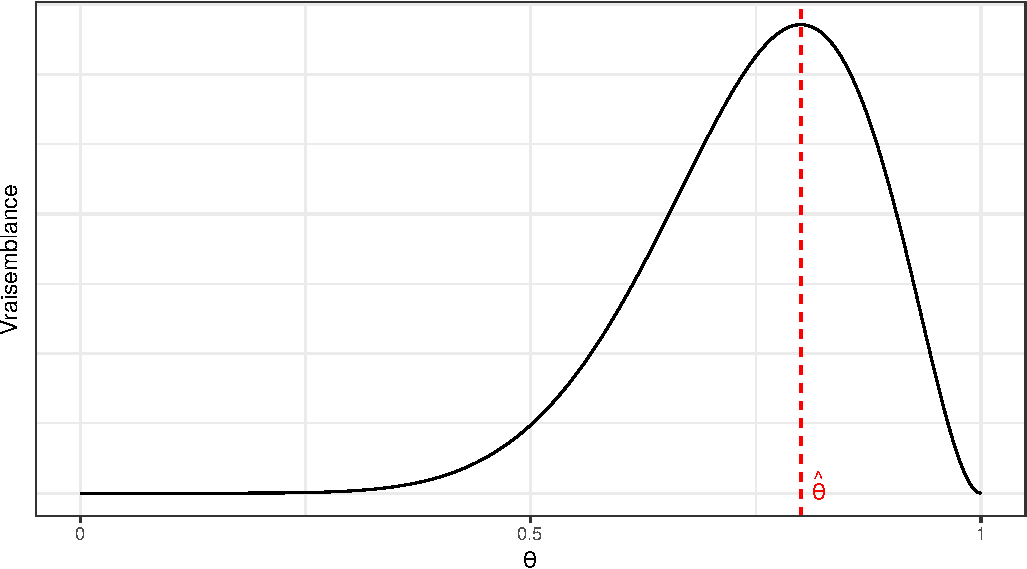
\includegraphics{diapos_inference_bayesienne_files/figure-beamer/vraisemblance_10-1.pdf}

\end{frame}

\begin{frame}{Vraisemblance pour \(n = 1000\) et 800 succès}
\protect\hypertarget{vraisemblance-pour-n-1000-et-800-succuxe8s}{}

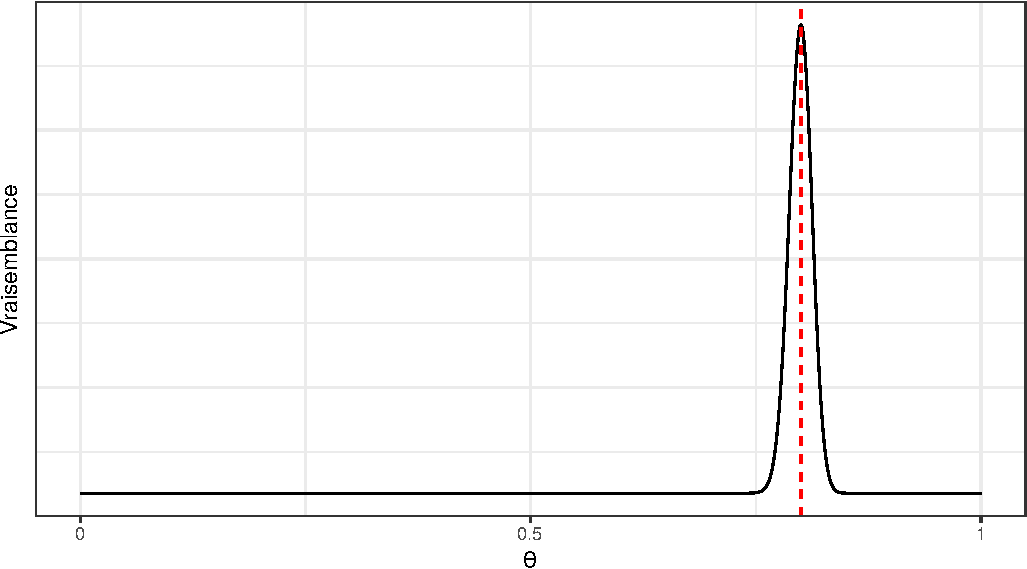
\includegraphics{diapos_inference_bayesienne_files/figure-beamer/vraisemblance_1000-1.pdf}

\end{frame}

\begin{frame}{Inférence bayésienne}
\protect\hypertarget{infuxe9rence-bayuxe9sienne}{}

\begin{block}{A priori sur \(\theta\)}

\begin{itemize}
\tightlist
\item
  On a potentiellement une connaissance \emph{a priori} sur \(\theta\).
  \pause
\item
  On peut modéliser cet \emph{a priori} sur le paramètre \(\theta\)
  (savoir expert\ldots{}) par une \textbf{variable aléatoire} de densité
  \(\pi(\theta)\). \pause 
\item
  Cette distribution est appelée \textbf{prior} sur \(\theta\).\pause
\item
  Dans ce contexte, \(\theta\) est un variable aléatoire, on dispose
  d'un \emph{a priori} sur sa loi.
\end{itemize}

\end{block}

\end{frame}

\begin{frame}{Exemples de loi a priori}
\protect\hypertarget{exemples-de-loi-a-priori}{}

Aucune idée sur \(\theta\)

\begin{center}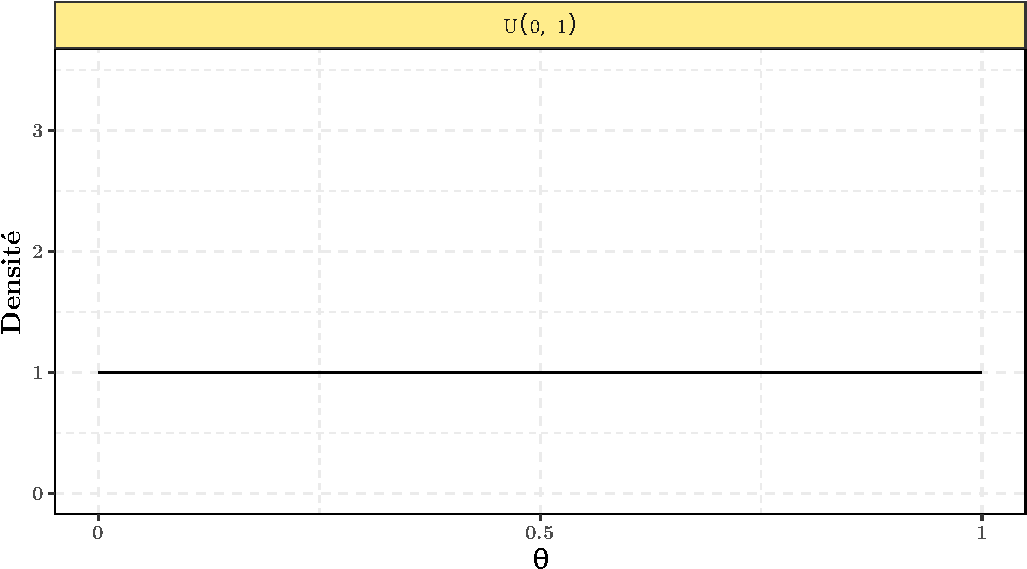
\includegraphics{diapos_inference_bayesienne_files/figure-beamer/plot_prior_unif-1} \end{center}

\textbf{Remarque} une loi \(\mathcal{U}[0, 1]\) est \textbf{strictement}
équivalente à une loi \(\mathcal{B}eta(1, 1)\).

\end{frame}

\begin{frame}{Exemples de loi a priori}
\protect\hypertarget{exemples-de-loi-a-priori-1}{}

A priori léger sur une pièce équitable

\begin{center}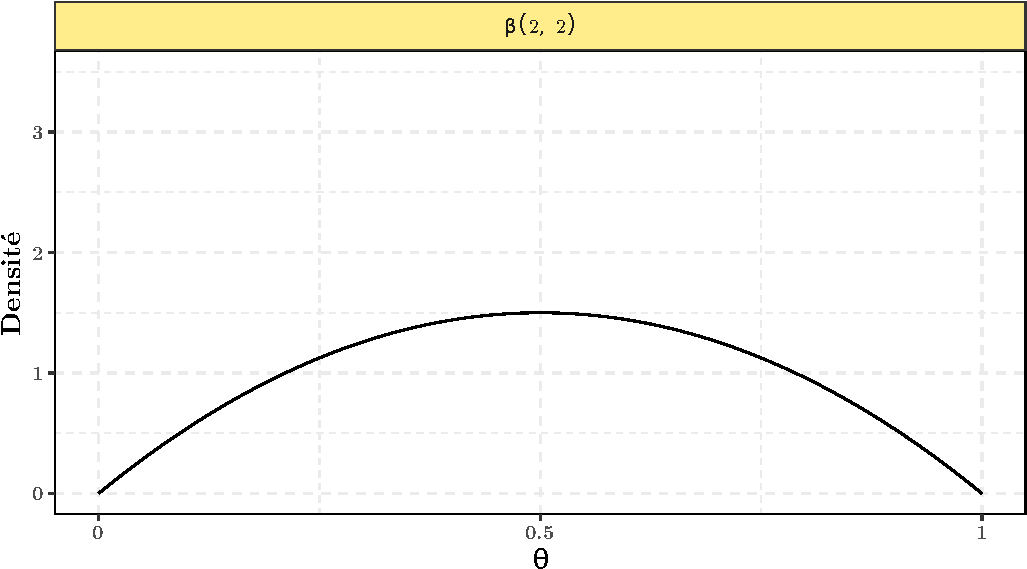
\includegraphics{diapos_inference_bayesienne_files/figure-beamer/plot_prior_beta_equil-1} \end{center}

\end{frame}

\begin{frame}{Exemples de loi a priori}
\protect\hypertarget{exemples-de-loi-a-priori-2}{}

A priori fort sur une pièce inéquitable

\begin{center}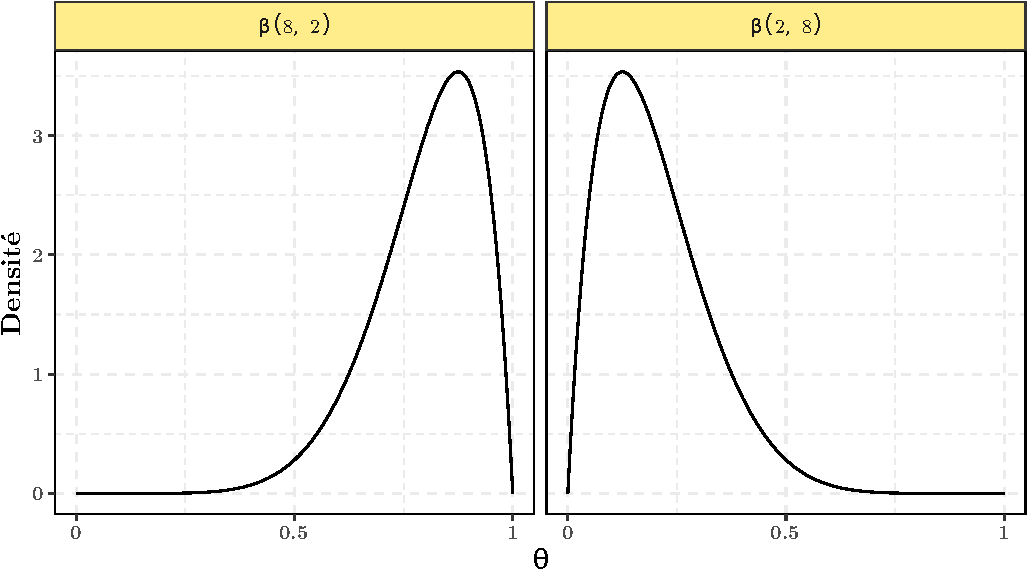
\includegraphics{diapos_inference_bayesienne_files/figure-beamer/plot_prior_beta_non_equil-1} \end{center}

\end{frame}

\hypertarget{infuxe9rence-bayuxe9sienne-1}{%
\section{Inférence bayésienne}\label{infuxe9rence-bayuxe9sienne-1}}

\begin{frame}{Inférence bayésienne}
\protect\hypertarget{infuxe9rence-bayuxe9sienne-2}{}

\begin{tabular}{cc}

\includegraphics[width = 0.5\textwidth, height=0.5\textwidth]{figures/formule_bayes_1.png}&
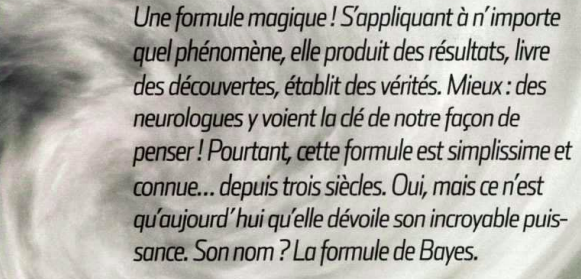
\includegraphics[width = 0.5\textwidth, height=0.5\textwidth]{figures/formule_bayes_2.png}
\end{tabular}

\end{frame}

\begin{frame}{Inférence bayésienne}
\protect\hypertarget{infuxe9rence-bayuxe9sienne-3}{}

\begin{block}{Influence des données, distribution a posteriori.}

\begin{itemize}
\tightlist
\item
  L'objectif est de l'inférence est de \textbf{connaître la distribution
  de \(\theta\) sachant les données}. \pause
\item
  La densité de cette distribution sur \(\theta\) est notée
  \(\pi(\theta \vert \mathbf{x})\), et est appelée \textbf{posterior} ou
  \textbf{loi a posteriori}.\pause
\item
  On \textbf{actualise} notre connaissance sur \(\theta\) grâce aux
  données.\pause
\end{itemize}

\end{block}

\begin{block}{Formule de Bayes}

\[\mathbb{P}(B\vert A) = \frac{P(A\vert B)\mathbb{P}(B)}{\mathbb{P}(A)}\]
\pause Dans le cas avec des densités: \[
\pi(\theta \vert x_{1:n}) = \frac{p(x_{1:n}, \theta)}{p(x_{1:n})} = \frac{L(x_{1:n} \vert \theta)\pi(\theta)}{p(x_{1:n})}
\] où \(p\) est notation surchargée pour les densités.

Cette relation est résumée par:
\[\pi(\theta \vert \mathbf{x}) \propto L(x_{1:n} \vert \theta)\pi(\theta)\]

\end{block}

\end{frame}

\begin{frame}{Objectif de l'inférence Bayésienne}
\protect\hypertarget{objectif-de-linfuxe9rence-bayuxe9sienne}{}

\[\pi(\theta \vert \mathbf{x}) \propto L(x_{1:n} \vert \theta)\pi(\theta)\]

L'inférence Bayésienne a pour but la détermination (exacte, ou par
simulation) du posterior \(\pi(\theta\vert \mathbf{x})\).

\end{frame}

\hypertarget{exemple-1-moduxe8le-avec-prior-conjuguuxe9}{%
\section{Exemple 1: modèle avec prior
conjugué}\label{exemple-1-moduxe8le-avec-prior-conjuguuxe9}}

\begin{frame}{Posterior dans le modèle \(\mathcal{B}eta\)-Binomial}
\protect\hypertarget{posterior-dans-le-moduxe8le-mathcalbeta-binomial}{}

On revient au cas de pile ou on face où
\[L(x_{1:n}\vert \theta) = \prod_{k = 1}^{n}\mathbb{P}_\theta(X = x_k) = \theta^{\sum_{k=1}^n x_k}\left(1 - \theta \right)^{n - \sum_{k=1}^n x_k}\]
\pause Pour l'inférence bayésienne, on pose comme \emph{a priori} que
\(\theta \sim \mathcal{B}eta(a, b)\), ainsi:
\[\pi(\theta) = \frac {\theta^{a -1}(1-\theta)^{b -1}}{\int _{0}^{1}u^{a -1}(1-u)^{b -1}\,du}\mathbf{1}_{0 < \theta < 1} \propto \theta^{a -1}(1-\theta)^{b -1}\mathbf{1}_{0 < \theta < 1}\]
On cherche la loi de \(\theta \vert x_{1:n}\).\pause \begin{align*}
\pi(\theta \vert x_{1:n}) &\propto L(x_{1:n}\vert \theta)\pi(\theta)\\
&\propto \theta^{\sum_{k=1}^n x_k}\left(1 - \theta \right)^{n - \sum_{k=1}^n x_k} \theta^{a -1}(1-\theta)^{b -1}\mathbf{1}_{0 < \theta < 1}\\
&\propto \theta^{a + \sum_{k=1}^n x_k - 1}(1-\theta)^{b + n - \sum_{k=1}^n x_k -1}\mathbf{1}_{0 < \theta < 1}
\end{align*} \pause On reconnaît que \(\pi(\theta\vert \mathbf{x})\) est
la densité d'une loi
\[\theta\vert x_{1:n} \sim \beta\left(a + \sum_{k = 1}^n x_k, b + n - \sum_{k = 1}^n x_k\right)\]

\end{frame}

\begin{frame}{Cas \(n = 10\) et 8 succès}
\protect\hypertarget{cas-n-10-et-8-succuxe8s}{}

\[\theta\vert x_{1:n} \sim \beta\left(a + \sum_{i}^n x_i, b + n - \sum_{i}^n x_i\right)\]

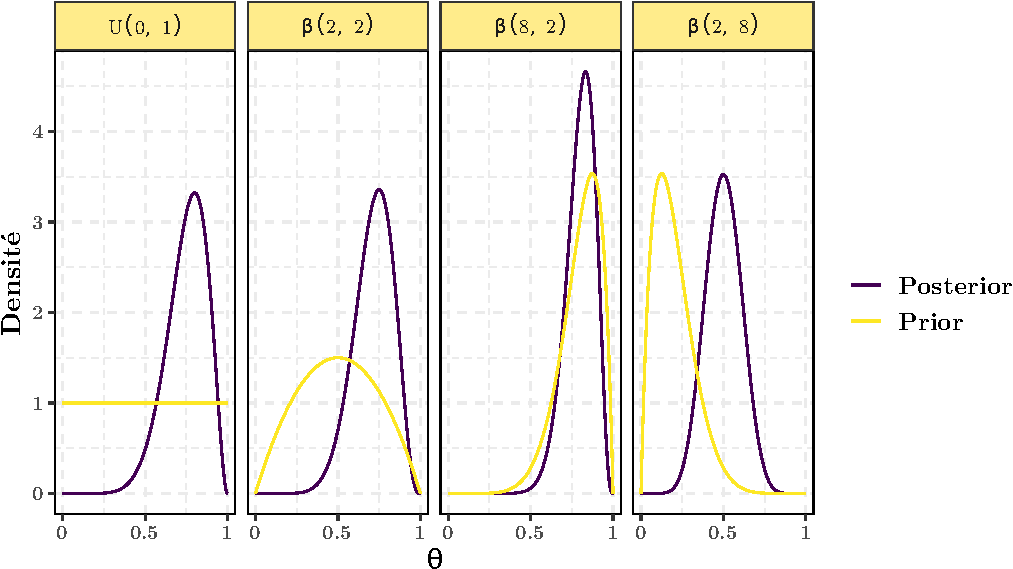
\includegraphics{diapos_inference_bayesienne_files/figure-beamer/plot_prior_posterior_small_samp-1.pdf}

\end{frame}

\begin{frame}{Cas \(n = 1000\) et 800 succès}
\protect\hypertarget{cas-n-1000-et-800-succuxe8s}{}

\[\theta\vert x_{1:n} \sim \beta\left(a + \sum_{i}^n x_i, b + n - \sum_{i}^n x_i\right)\]

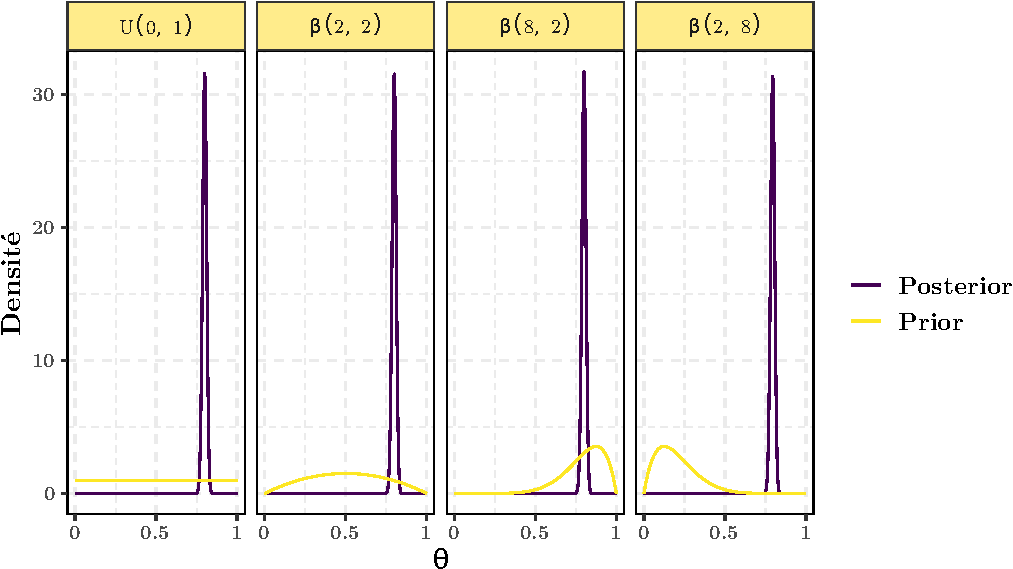
\includegraphics{diapos_inference_bayesienne_files/figure-beamer/plot_prior_posterior_large_samp-1.pdf}

\end{frame}

\begin{frame}{Prior conjugué}
\protect\hypertarget{prior-conjuguuxe9}{}

Pour les modèles basés sur une vraisemblance ``classique'', certains
priors ont des priorités de conjugaison. Pour un modèle Bayésien, on
appelle prior conjugué un prior \(\pi(\theta)\) tel que le posterior
\(\pi(\mathbf{x}\vert \theta)\) est dans la même famille de loi que
\(\pi(\theta)\).

\begin{block}{Exemples}

\begin{itemize}
\tightlist
\item
  Modèle Bernouilli-Beta;
\item
  Modèle Gaussien (prior: Normal Inverse Gamma);
\item
  Modèle à densités dans la famille exponentielle.
\end{itemize}

\end{block}

\begin{block}{Intérêt}

L'inférence est directe!

\end{block}

\end{frame}

\hypertarget{choix-de-prior-et-estimateurs-bayuxe9siens}{%
\section{Choix de prior et estimateurs
Bayésiens}\label{choix-de-prior-et-estimateurs-bayuxe9siens}}

\begin{frame}{Influence et choix du prior}
\protect\hypertarget{influence-et-choix-du-prior}{}

Pour un nombre de données limité, la \textbf{forme du prior} a un impact
sur la forme du posterior.

\pause

\begin{block}{Choix du prior}

La forme du prior peut être choisie en fonction du \emph{savoir expert}
(littérature existante, expériences passées).

\textbf{ATTENTION:} Le support du posterior sera toujours inclu dans le
support du prior.

\pause

Si le prior charge tout le support de manière égale, on dit qu'il est
\textbf{non informatif}.

\end{block}

\begin{block}{Prior impropre}

Si le support de \(\theta\) est sur \(\mathbb{R}\), un prior non
informatif est une ``uniforme sur \(\mathbb{R}\)''. Ceci n'est pas une
loi. \pause

On peut cependant noter abusivement \(\pi(\theta) \propto 1\). Dans ce
cas, si
\(\frac{L(x_{1:n} \vert \theta)}{\int L\left(x_{1:n} \vert \theta\right)\text{d} \theta}\)
définit une loi de probabilité en \(\theta\), alors le posterior
\(\pi(\theta\vert \mathbf{x})\) est bien défini.

\begin{itemize}
\tightlist
\item
  Le prior est alors dit \textbf{impropre}.
\end{itemize}

\end{block}

\end{frame}

\begin{frame}{Choix du prior}
\protect\hypertarget{choix-du-prior-1}{}

\begin{block}{Exemple de prior impropre.}

On suppose que \(\mathbf{x}\) est issu d'un échantillon i.i.d. de taille
\(n\), de loi \(\mathcal{N}(\mu, 1)\) où \(\mu\) est inconnu. N'ayant
aucune idée de la valeur de \(\mu\), on prend un prior non informatif.
On a alors: \begin{align*}
\pi(\mu \vert x_{1:n}) &\propto L(x_{1:n} \vert \theta)\\
&\propto \text{e}^{-\frac{1}{2}\sum_{k = 1}^n (x_k - \mu)^2}\\
&\propto\text{e}^{-\frac{1}{2}(n \mu^2 - 2\mu\sum_{k = 1}^n x_k)}\\
&\propto\text{e}^{-\frac{n}{2}(\mu - \frac{1}{n}\sum_{k = 1}^n x_k)^2}
\end{align*} Ainsi,
\[\mu\vert x_{1:n} \sim \mathcal{N}\left(\frac{1}{n}\sum_{k = 1}^n x_k, \frac{1}{n}\right)\]

\end{block}

\end{frame}

\begin{frame}{Estimateurs Bayésiens}
\protect\hypertarget{estimateurs-bayuxe9siens}{}

\begin{block}{Maximum a posteriori (MAP)}

Reprenant l'idée du MLE, il s'agit du mode de la distribution a
posteriori:

\[MAP(\theta \vert x_{1:n}) = \text{argmax}_\theta \pi(\theta \vert x_{1:n})\]
\pause

\end{block}

\begin{block}{Exemple sur la modèle Beta binomial}

\[\theta\vert x_{1:n} \sim \beta\left(a + \sum_{k = 1}^n x_k, b + n - \sum_{k = 1}^n x_k\right)\]
On peut montrer que, pour \(a + b + n > 2\) et
\(a + \sum_{k = 1}^n x_k \geq 1\)
\[MAP(\theta \vert x_{1:n}) = \frac{a + \sum_{k = 1}^n x_k-1}{a  +  b + n -2}\]
\pause On remarque que pour \(a = b = 1\) (prior uniforme), il s'agit du
maximum de vraisemblance, et que cela tend vers le MV quand \(n\)
grandit.

\end{block}

\end{frame}

\begin{frame}{Estimateurs Bayésiens}
\protect\hypertarget{estimateurs-bayuxe9siens-1}{}

\begin{block}{Espérance a posteriori}

Soit un modèle Bayésien paramétré par une vraie valeur
\(\theta^* \in \Theta\) et de prior \(\pi(\theta)\) Pour toute fonction
\(\varphi\), la variable aléatoire
\[\mathbb{E}[\varphi(\theta) \vert \mathbf{X}]\] est un estimateur
Bayésien de \(\varphi(\theta^*)\). \pause

Par exemple, pour un échantillon observé \(\mathbf{x}\), une estimation
bayésienne possible de \(\theta^*\) est
\[\hat{\theta} = \mathbb{E}[\theta \vert \mathbf{X} = x_{1:n}] = \int_\Theta \theta \pi(\theta \vert x_{1:n}) \text{d}\theta\]

\end{block}

\begin{block}{Exemple sur la modèle Beta-Binomial}

Pour un prior \(\beta(a, b)\), on a
\[\hat{\theta} \overset{\text{loi } \beta}{=} \frac{a + \sum_{i = 1}^n x_i}{a + b + n} = \underbrace{\frac{n}{a + b + n}}_{\text{Poids données}}\times \overbrace{\frac{\sum_{i=1}^n x_i}{n}}^{\text{Max. de vrais.}} + \underbrace{\frac{a + b}{a + b + n}}_{\text{Poids prior}} \times \overbrace{\frac{a}{a + b}}^{\mathbb{E}\text{ du prior}}\]

\end{block}

\end{frame}

\begin{frame}{Estimateurs Bayésiens}
\protect\hypertarget{estimateurs-bayuxe9siens-2}{}

\begin{block}{Intervalle de crédibilité}

Pour toute région \(\mathcal{R} \subset \Theta\), on peut quantifier:
\[\mathbb{P}(\theta \in \mathcal{R} \vert  \mathbf{X} = x_{1:n}) = \int_\mathcal{R} \pi(\theta \vert x_{1:n}) \text{d}\theta\]
Pour \(\alpha \in ]0, 1[\), une région de crédibilité de niveau
\(1-\alpha\) est une région \(\mathcal{R} \subset \Theta\) telle que
\[\mathbb{P}(\theta \in \mathcal{R} \vert  \mathbf{X} = x_{1:n}) = 1 - \alpha\]
Cet intervalle n'est pas asymptotique, mais \textbf{dépend du prior}.

\textbf{Remarque}, ici l'aléa est bien sur \(\theta\) (contrairement à
un intervalle de confiance).

\end{block}

\end{frame}

\begin{frame}{Intervalles de crédibilités (centrés) à 95\% dans le
modèle Beta binomial}
\protect\hypertarget{intervalles-de-cruxe9dibilituxe9s-centruxe9s-uxe0-95-dans-le-moduxe8le-beta-binomial}{}

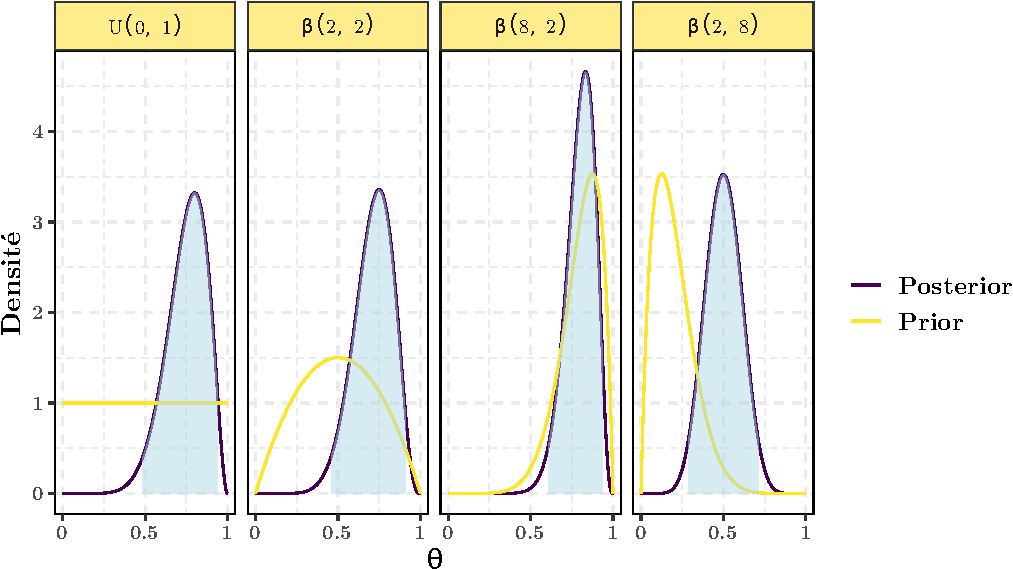
\includegraphics{diapos_inference_bayesienne_files/figure-beamer/intervalle_credi-1.pdf}

\end{frame}

\hypertarget{exemple-2-cas-non-conjuguuxe9}{%
\section{Exemple 2: cas non
conjugué}\label{exemple-2-cas-non-conjuguuxe9}}

\begin{frame}{Exemple: Prédiction de présence d'oiseaux}
\protect\hypertarget{exemple-pruxe9diction-de-pruxe9sence-doiseaux}{}

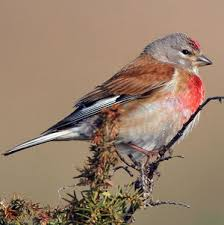
\includegraphics[width = 0.3\textwidth]{figures/linotte.jpeg}

Une étude consiste en l'observation de la présence ou non de la linotte
mélodieuse sur différents sites échantillonnés.

\begin{block}{Caractéristiques des sites}

Sur ces différents sites sont mesurées différentes caractéristiques:

\begin{itemize}
\tightlist
\item
  Le nombre de vers moyens sur une surface au sol de \(1m^2\).
  (Covariable 1)
\item
  La hauteur d'herbe moyenne sur une surface au sol de \(1m^2\).
  (Covariable 2)
\item
  On calcule cette hauteur d'herbe au carré. (Covariable 3).
\end{itemize}

\end{block}

\end{frame}

\begin{frame}{Données}
\protect\hypertarget{donnuxe9es}{}

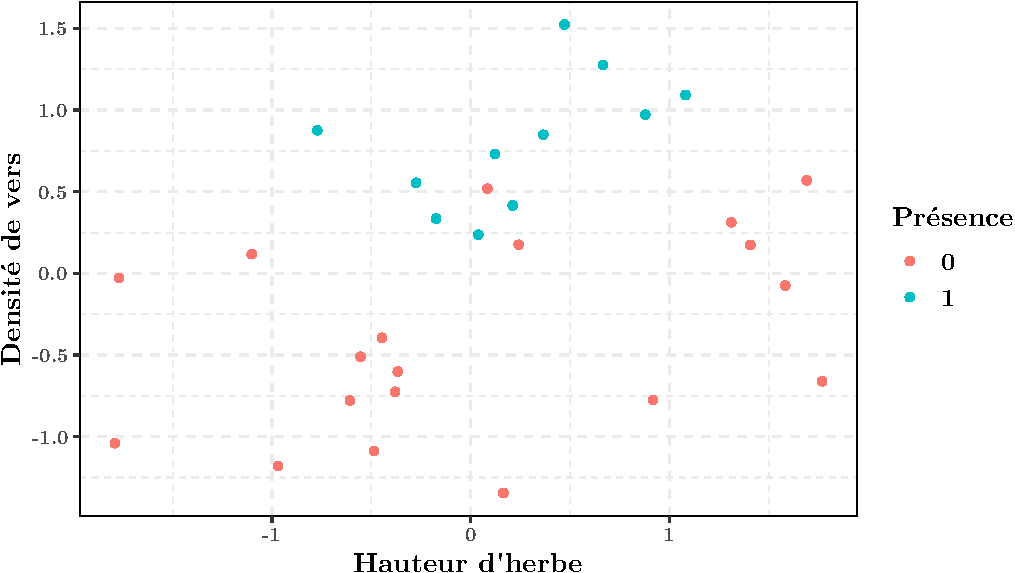
\includegraphics{diapos_inference_bayesienne_files/figure-beamer/plot_donnees_presence-1.pdf}

\end{frame}

\begin{frame}{Notations et modèle de régression probit}
\protect\hypertarget{notations-et-moduxe8le-de-ruxe9gression-probit}{}

On note \(y_1, \dots, y_n\) les observations de présence (1 si on
observe un oiseau, 0 sinon) sur les sites \(1\) à \(n\).

On note
\[\mathbf{x}_k = (\overset{\text{Nb. vers}}{x_{k,1}}, \overset{\text{Haut. herbe}}{x_{k,2}}, \overset{\text{Haut. herbe}^2}{x_{k,3}})^T\]
le vecteur des covariables sur le \(k\)-ème site
\((1\leq k \leq n)\).\pause

On pose le modèle suivant:

\(Y_k \sim \mathcal{B}ern(p_k)\) où
\[p_k = \phi(\beta_0 + \beta_1 x_{i1} + \beta_2x_{i2} + \beta_3 x_{i3}) = \phi(\mathbf{x}_k^T\theta),\]
où

\begin{itemize}
\tightlist
\item
  \(\phi\) est la fonction de répartition d'une \(\mathcal{N}(0, 1)\),
  i.e.
  \[\phi(z) = \frac{1}{\sqrt{2\pi}}\int_{-\infty}^z \text{e}^{-\frac{u^2}{2}}\text{d}u\]
\item
  \(\theta = \left\lbrace \beta_0, \beta_1, \beta_2, \beta_3\right\rbrace\)
  est le vecteur des paramètres à estimer.
\end{itemize}

\end{frame}

\begin{frame}{Modèle Bayésien}
\protect\hypertarget{moduxe8le-bayuxe9sien}{}

\begin{block}{Prior sur \(\theta\)}

Comme a priori sur \(\theta\), on choisit une normale avec une grande
variance\(\theta \overset{\text{prior}}{\sim} \mathcal{N}(0, 4 I),\)
donc
\[\pi(\theta) = \frac{1}{\sqrt{2\pi \times 4}^4} \text{e}^{-\frac{1}{8}\theta^T\theta}\]
où \(I\) est la matrice Identité (ici \(4 \times 4\)) \pause

\end{block}

\begin{block}{Vraisemblance}

Pour un vecteur d'observations \(y_{1:k}\), la vraisemblance
\[L(y_{1:n}\vert \theta) = \prod_{k = 1}^n \underset{\text{Proba. présence}}{\phi(\mathbf{x}_k^T\theta)^{y_k}}\times \underset{\text{Proba. absence}}{(1 - \phi(\mathbf{x}_k^T\theta))}^{1 - y_k}\]
\pause

\end{block}

\begin{block}{Posterior}

Le posterior est donc donné par:
\[\pi(\theta \vert \mathbf{x}) \propto \pi(\theta) L(y_{1:n}\vert \theta) \propto \frac{1}{64\pi^2}\text{e}^{-\frac{1}{8}\theta^T\theta} \prod_{k = 1}^n \phi(\mathbf{x}_k^T\theta)^{y_k} (1 - \phi(\mathbf{x}_k^T\theta))^{1 - y_k}\]

\end{block}

\end{frame}

\begin{frame}{Posterior modèle Normal-Probit}
\protect\hypertarget{posterior-moduxe8le-normal-probit}{}

\[\pi(\theta \vert y_{1:n}) \propto \pi(\theta) L(y_{1:n}\vert \theta) \propto \frac{1}{64\pi^2}\text{e}^{-\frac{1}{8}\theta^T\theta} \prod_{k = 1}^n \phi(\mathbf{x}_k^T\theta)^{y_k} (1 - \phi(\mathbf{x}_k^T\theta))^{1 - y_k}\]

Cette densité n'est pas standard:

\begin{itemize}
\tightlist
\item
  On ne sait pas calculer des espérances associées (estimateurs
  bayésiens);
\item
  On pourrait approcher ces espérances par méthodes de Monte Carlo\pause
\item
  Encore faut il savoir simuler!\pause
\item
  Le cas où le posterior ne fait pas partie d'une famille connue est
  très fréquent.
\item
  L'inférence bayésienne est une motivation énorme pour les algos de
  simulations de loi.
\end{itemize}

\end{frame}

\begin{frame}{Simulation posterior modèle Normal-Probit}
\protect\hypertarget{simulation-posterior-moduxe8le-normal-probit}{}

On veut simuler selon
\[\pi(\theta \vert y_{1:n}) \propto \only<4->{\overbrace}{\frac{1}{64\pi^2}\text{e}^{-\frac{1}{8}\theta^T\theta} \prod_{k = 1}^n \phi(\mathbf{x}_k^T\theta)^{y_k} (1 - \phi(\mathbf{x}_k^T\theta))^{1 - y_k}}^{\only<4->{\tilde{\pi}(\theta\vert y_{1:n})}} \]
\pause

\begin{block}{Simulation par acceptation rejet}

On voudrait simuler selon \(\pi(\theta \vert y_{1:n})\).\pause

\begin{itemize}
\item
  Idée 1: trouver une densité \(g\) selon laquelle on sait simuler et
  telle qu'il existe \(M>0\) tel que
  \[\forall \theta \in \mathbb{R}^4,~\frac{\pi(\theta \vert y_{1:n})}{g(\theta)} \leq M\]
  \pause Mais \(\pi(\theta \vert y_{1:n})\) n'est connu qu'a une
  constante près!
  \[\pi(\theta \vert y_{1:n}) = \frac{\tilde{\pi}(\theta \vert y_{1:n})}{\int_{\mathbb{R}^4}\pi(u) L(y_{1:n}\vert u) \text{d} u}\]
\item
  \textbf{Rappel} L'acceptation rejet marche toujours si on ne connait
  la loi cible qu'à une constante près! (voir TD pour la preuve).
\end{itemize}

\end{block}

\end{frame}

\begin{frame}{Simulation posterior modèle Normal-Probit}
\protect\hypertarget{simulation-posterior-moduxe8le-normal-probit-1}{}

On veut simuler selon
\[\pi(\theta \vert y_{1:n}) \propto \overbrace{\frac{1}{64\pi^2}\text{e}^{-\frac{1}{8}\theta^T\theta} \prod_{k = 1}^n \phi(\mathbf{x}_k^T\theta)^{y_k} (1 - \phi(\mathbf{x}_k^T\theta))^{1 - y_k}}^{\tilde{\pi}(\theta\vert y_{1:n})} \]

\begin{itemize}
\tightlist
\item
  Idée 2: trouver une densité \(g\) selon laquelle on sait simuler et
  telle qu'il existe \(M>0\) tel que
  \[\forall \theta \in \mathbb{R}^4,~\frac{\tilde{\pi}(\theta \vert y_{1:n})}{g(\theta)} \leq M\]
\end{itemize}

\end{frame}

\begin{frame}{Implémentation de l'acceptation rejet}
\protect\hypertarget{impluxe9mentation-de-lacceptation-rejet}{}

On peut par exemple prend pour \(g\) la densité correspondant au prior
(\(g(\theta) = \pi(\theta)\)). On remarque que dans ce cas
\[\frac{\tilde{\pi}(\theta \vert y_{1:n})}{g(\theta)} = \frac{\pi(\theta)L(y_{1:n}\vert \theta)}{\pi(\theta)} = \prod_{k = 1}^n \phi(\mathbf{x}_k^T\theta)^{y_k} (1 - \phi(\mathbf{x}_k^T\theta))^{1 - y_k} \leq 1 =:M\]
\textbf{Remarque:} il existe un \(M\) optimal plus petit que 1. \pause

\begin{block}{Algorithme de simulation selont
\(\pi(\theta\vert y_{1:n})\)}

\begin{enumerate}
\tightlist
\item
  On tire \(\theta_{cand} \sim \mathcal{N}(0, 4I)\)
\item
  On tire (independamment) \(U\sim \mathcal{U}[0, 1]\)
\item
  Si \(U < \frac{L(y_{1:n}\vert \theta)}{M}\), on accepte
  \(\theta_{cand}\)
\item
  Sinon on recommence
\end{enumerate}

\pause

\textbf{Remarque}, l'échantillon obtenu est tiré selon \emph{la loi
jointe} (on ne tire pas \(\beta_0\) puis \(\beta_1\), etc\ldots{})

\end{block}

\end{frame}

\begin{frame}{Echantillon du posterior, et loi a posteriori marginales}
\protect\hypertarget{echantillon-du-posterior-et-loi-a-posteriori-marginales}{}

On effectue un tirage de taille \(M = 1000\)

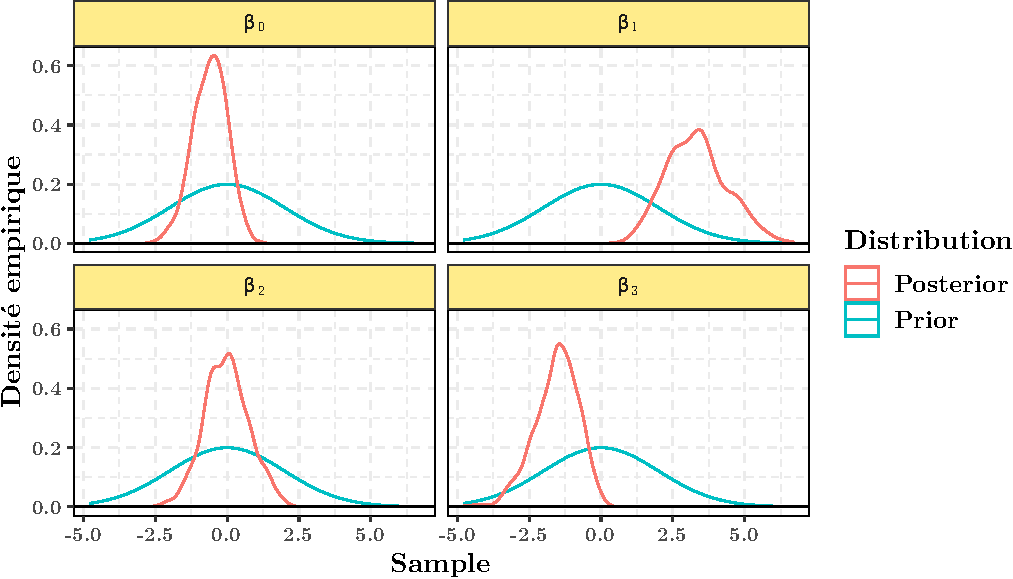
\includegraphics{diapos_inference_bayesienne_files/figure-beamer/plot_posterior_samples-1.pdf}

\begin{itemize}
\tightlist
\item
  Les données ont bien actualisé la connaissance sur \(\theta\)
\end{itemize}

\end{frame}

\begin{frame}{Echantillon du posterior et loi jointe}
\protect\hypertarget{echantillon-du-posterior-et-loi-jointe}{}

On peut regarder la loi jointe de \((\beta_0,\beta_1 \vert y_{1:n})\):

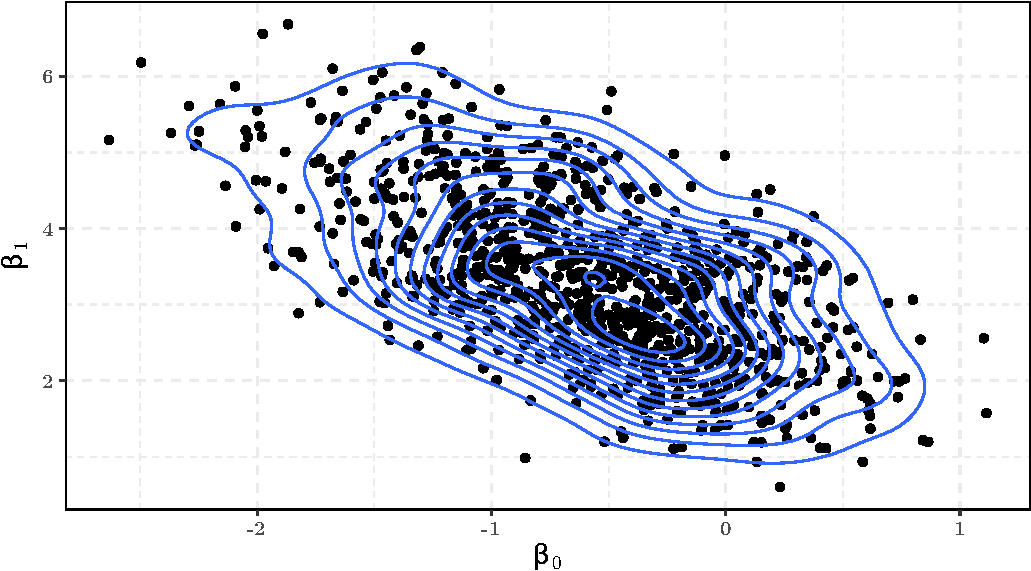
\includegraphics{diapos_inference_bayesienne_files/figure-beamer/loi_jointe_beta0_beta1-1.pdf}

\end{frame}

\begin{frame}{Estimateurs bayésiens}
\protect\hypertarget{estimateurs-bayuxe9siens-3}{}

On prend comme estimateur l'espérance \textbf{a posteriori}. De plus, on
regarde l'estimation de l'intervalle

\begin{longtable}[]{@{}lrrr@{}}
\toprule
Parameter & Estimation & inf\_IC95 & sup\_IC95\tabularnewline
\midrule
\endhead
beta{[}0{]} & -0.595 & -1.868800 & 0.5265336\tabularnewline
beta{[}1{]} & 3.329 & 1.441659 & 5.5525325\tabularnewline
beta{[}2{]} & -0.019 & -1.499485 & 1.5197882\tabularnewline
beta{[}3{]} & -1.551 & -3.222323 & -0.2565622\tabularnewline
\bottomrule
\end{longtable}

\end{frame}

\begin{frame}{Au delà de l'acceptation rejet}
\protect\hypertarget{au-deluxe0-de-lacceptation-rejet}{}

Dans le cas précédent, l'espérance du temps d'attente avant une
acceptation est donnée par
\[\frac{M}{\int L(y_{1:n}\vert \theta)\pi(\theta) \text{d}\theta}\]

\pause

Mécaniquement, cette quantité augmente quand \(n\) augmente, et
l'acceptation rejet dvient prohibitif.

En pratique, l'inférence Bayésienne utilisera d'autres algorithmes de
simulations de loi: les algorithmes de Monte Carlo par chaîne de Markov.

\end{frame}

\end{document}
